\RequirePackage{cmap}
\documentclass[aps,pra,reprint,nofootinbib,floatfix,longbibliography]{revtex4-2}

\usepackage[T1]{fontenc}
\usepackage[utf8]{inputenc}
\input{glyphtounicode}
\pdfgentounicode=1
\usepackage{lmodern}
\usepackage{microtype}
\emergencystretch=1.5em
\usepackage{amsmath,amssymb,amsfonts,amsthm,mathtools}
\usepackage{bm}
\usepackage{graphicx}
\usepackage{booktabs}
\usepackage{xcolor}
\usepackage[colorlinks=true,linkcolor=blue!70!black,citecolor=blue!70!black,urlcolor=blue!70!black]{hyperref}

% Mathematical macros
\newcommand{\braket}[2]{\langle #1 | #2 \rangle}
\newcommand{\ket}[1]{| #1 \rangle}
\newcommand{\bra}[1]{\langle #1 |}
\newcommand{\norm}[1]{\lVert #1 \rVert}
\newcommand{\abs}[1]{\lvert #1 \rvert}

\begin{document}

\title{Overcompleteness and Continuous Frame Properties of Physical Perfect Vortex Beams.\\II. Classical and Quantum Optical Applications}

\author{Sebasti\'an Ayala}
\email{ayala.phys.ds@gmail.com}
\homepage{https://orcid.org/0009-0003-7348-3883}
\affiliation{Independent Researcher, Cauquenes, Chile}

\date{November 19, 2026}

\begin{abstract}
In the companion paper~[Paper~I], we established that finite-width physical perfect optical vortex beams (PVBs) form a continuous Bessel system on $L^2(\mathbb{R}^2)$ with isotropic Gaussian convolution frame operator $S_w = G_w * \cdot$, sharp Paley--Wiener frame bounds on bandlimited optical subspaces $\mathcal{H}_{k_{\max}}$, an exact $(p+1)$-term closed-form Laguerre--Gaussian ($\mathrm{LG}_{p,l}$) expansion $c_{l,p}(R)$, and monotonically well-conditioned unit-normalized discrete radial Gram matrices. Here, we translate this operator framework into five quantitative protocols across classical and quantum photonics: (i) Tikhonov-regularized Paley--Wiener modal deconvolution under bandlimited additive white Gaussian noise, achieving a $258.6\times$ ($24.1\,\mathrm{dB}$) mean-square-error reduction on noisy $\mathrm{LG}_{2,1}$ fields ($\mathrm{SNR} = 20\,\mathrm{dB}$, $w/w_0 = 0.25$, $w k_{\max} = 3.0$, $\alpha_{\mathrm{reg}}^{\mathrm{opt}} = 0.04902$); (ii) telecom ring-core fiber (RCF) Sturm--Liouville waveguide coupling ($98.52\%$ mean efficiency across $l = 0\text{--}8$ and $+6.90\,\mathrm{dB}$ gain over fixed-collimator $\mathrm{LG}_{0,4}$, matching the $+6.83\,\mathrm{dB}$ experimental benchmark of Villalba \emph{et al.}) combined with $N = 6$ concentric multi-ring space-division multiplexing incurring $\le 0.42\,\mathrm{dB}$ zero-forcing noise penalty at $\Delta R = 2.0\,w$; (iii) single-OAM discrete PVB dual-frame spatial filtering in Kolmogorov turbulence, suppressing field error by $4.24\times$ at $D/r_0 = 3.0$ by rejecting all $l \neq l_0$ azimuthal crosstalk; (iv) passive single-shot $M = 5$ Gouy-diverse informationally complete POVM (IC-POVM) tomography of $d = 4$ radial qudits (lifting single-plane rank $7/16$ to full rank $16/16$ with superoperator condition number $\kappa(\mathcal{S}_{\mathrm{POVM}}) = 442.5$ and single-photon Cram\'er--Rao bound $41.80$); and (v) $l$-invariant quantum-key-distribution pupil transmission and leading-order circular-iris Bell--CHSH entanglement preservation [$2\sqrt{2} - S_{\mathrm{PVB}}(R_0) \le 6.5\times 10^{-6}$ at $w/R_0 = 0.1$, versus $S_{\mathrm{LG}}(R_0) = 2.0008$].
\end{abstract}

\maketitle

\section{Introduction}
\label{sec:intro}

Structured optical beams carrying orbital angular momentum (OAM)~\cite{Allen1992,Siegman1986,Padgett2011} underpin high-capacity space-division multiplexing (SDM) in fibers and free space~\cite{Bozinovic2013,Willner2015,Wang2019} as well as high-dimensional quantum key distribution (QKD) and entanglement certification~\cite{Cerf2002,Mirhosseini2015,Bavaresco2018,Erhard2018}. Across all of these architectures, however, the $l$-dependent radial expansion $r_{\mathrm{rms}} = w_0\sqrt{2p+\abs{l}+1}$ of standard Laguerre--Gaussian ($\mathrm{LG}_{p,l}$) modes introduces severe mode-dependent aperture clipping, asymmetric waveguide insertion loss in fixed-annulus ring-core fibers (RCFs)~\cite{Ramachandran2009,Brunet2014,Gregg2015,Canas2021,RojasRojas2021}, and detection-efficiency side-channels in quantum receivers. Physical perfect optical vortex beams (PVBs)~\cite{Ostrovsky2013,Vaity2015,Reddy2016} overcome this geometric bottleneck by confining all topological charges $l \in \mathbb{Z}$ to a common ring radius $R > 0$ of finite annular half-width $w > 0$, enabling recent telecom RCF transmission demonstrations~\cite{Villalba2023} and partial-coherence modal analyses~\cite{Ferreira2026}.

Deploying physical PVBs as a complete modal toolkit—rather than merely as single-ring intensity carriers—requires accounting rigorously for their radial nonorthogonality and Gaussian frame smoothing. In the companion paper (Paper~I)~\cite{AyalaPaperI}, we proved that finite-width PVBs form a continuous Bessel family on $L^2(\mathbb{R}^2)$ with isotropic Gaussian convolution frame operator $S_w = G_w * \cdot$, sharp Paley--Wiener stability bounds on bandlimited subspaces $\mathcal{H}_{k_{\max}}$~\cite{Duffin1952,Daubechies1990,Ali1993,Christensen2016,PaulsenRaghupathi2016}, a Tikhonov-regularized canonical dual $S_{w,\alpha_{\mathrm{reg}}}^{-1}$, an exact $(p+1)$-term closed-form expansion $c_{l,p}(R)$ for all $\mathrm{LG}_{p,l}$ modes ($p \ge 0$), and well-conditioned unit-normalized discrete radial Gram matrices $[\gamma]_{nm}$.

In this second part, we demonstrate how each operator property from Paper~I~\cite{AyalaPaperI} translates directly into a concrete, quantitatively benchmarked protocol in classical or quantum optics: (i) regularized noisy deconvolution of multi-ring $\mathrm{LG}_{p,l}$ wavefields; (ii) Sturm--Liouville RCF launch optimization and concentric multi-ring SDM equalization using multi-plane light conversion (MPLC) or radial mode sorters~\cite{Fontaine2019,Berkhout2010,Bouchard2018,Proakis2008}; (iii) single-OAM discrete PVB dual-frame spatial filtering through Kolmogorov atmospheric turbulence~\cite{Paterson2005,TylerBoyd2009,AndrewsPhillips2005,Lane1992}; (iv) passive single-shot multi-plane Gouy-diverse informationally complete POVM (IC-POVM) tomography~\cite{Renes2004,Lvovsky2004} of radial photonic qudits; and (v) circular-iris Bell--CHSH entanglement preservation~\cite{Clauser1969,LawEberly2004,Walborn2010}. As in Paper~I, all physical models, boundary-value formulations, and optical benchmarks were conceived and audited under a strict Human-in-the-Loop (HITL) scientific protocol~\cite{Messeri2024,OToole2024,Chandra2026TheoPhysEval,Thorp2023Science,COPE2023AI}, with generative computational assistance disclosed in the Acknowledgments.

The remainder of this paper is organized as follows. Section~\ref{sec:summary} summarizes the PVB frame primitives from Paper~I and establishes the telecom $2f$ generation benchmark. Section~\ref{sec:classical_sdm} presents noisy Tikhonov modal reconstruction (Sec.~\ref{subsec:noisy_lg21}) and Sturm--Liouville RCF coupling with multi-ring SDM equalization (Sec.~\ref{subsec:rcf_sdm}). Section~\ref{sec:turbulence} analyzes single-OAM discrete PVB dual-frame filtering in Kolmogorov turbulence. Section~\ref{sec:quantum} develops passive Gouy-diverse radial-qudit IC-POVM tomography (Sec.~\ref{subsec:povm}) and circular-iris Bell--CHSH entanglement protection (Sec.~\ref{subsec:spdc_chsh}). Section~\ref{sec:conclusions} concludes the paper, and Appendix~\ref{app:methods} details the Sturm--Liouville solver, superoperator Fisher matrix, and iris asymptotics.

\section{Summary of PVB Frame Primitives and Telecom Generation Bridge}
\label{sec:summary}

Following the scaling convention of Paper~I~\cite{AyalaPaperI}, the continuous PVB frame elements at focal waist $z = 0$ are
\begin{equation}
\Phi_{l,R}(r,\phi) = C_0 e^{il\phi} \exp\!\left(-\frac{r^2 + R^2}{w^2}\right) I_{\abs{l}}\!\left(\frac{2Rr}{w^2}\right),
\label{eq:pvb_frame_def}
\end{equation}
with $C_0 = \sqrt{2/\pi}/w^2$ fixing the optimal Bessel upper bound $B = 1$ under measure $d\mu(l,R) = R\,dR$, whereas physical single-channel overlaps and discrete channel matrices use the unit-$L^2$-normalized states $\psi_{l,R} = \Phi_{l,R}/\norm{\Phi_{l,R}}_{L^2}$, where $\norm{\Phi_{l,R}}_{L^2}^2 = w^{-2} e^{-R^2/w^2} I_{\abs{l}}(R^2/w^2)$~\cite{Gradshteyn2014}. Generated via a $2f$ Fourier lens of focal length $f$ from a Bessel--Gaussian input of conical wavevector $k_r$ and Gaussian waist $w_g$~\cite{Vaity2015,Gori1987}, the ring parameters obey $R = k_r f/k_0$ and $w = 2f/(k_0 w_g)$ ($k_0 = 2\pi/\lambda$), separating pre-focal conical Bessel--Gauss self-healing ($z_{\mathrm{heal}} \approx k_0 a_{\mathrm{obs}}/k_r \le f$) from post-focal annular diffraction ($z_R^{\mathrm{ring}} = k_0 w^2/2$)~\cite{Reddy2016,AyalaPaperI}.

In telecom RCF experiments using phase-only spatial light modulators (SLMs), Rojas-Rojas \emph{et al.} predicted $>99.5\%$ modal coupling~\cite{RojasRojas2021}, and Villalba \emph{et al.} experimentally demonstrated across $l = 1\text{--}6$ a $15\times$ reduction in ring-radius variance, a $+6.83\,\mathrm{dB}$ coupling gain over $\mathrm{LG}$ modes at $l = 4$, and $1\,\mathrm{Gbps}$ transmission over $300\,\mathrm{m}$ of RCF~\cite{Villalba2023}. At telecom wavelength $\lambda = 1550\,\mathrm{nm}$ ($k_0 = 4.054\times 10^6\,\mathrm{m}^{-1}$), collection numerical aperture $\mathrm{NA} = 0.20$ ($k_{\max} = k_0\mathrm{NA} = 8.107\times 10^5\,\mathrm{m}^{-1}$), and RCF-matched half-width $w = 1.72\,\mu\mathrm{m}$, the dimensionless space--bandwidth parameter is $w k_{\max} = 1.394$. By Theorem~1 of Paper~I~\cite{AyalaPaperI}, projected PVBs on the Paley--Wiener subspace $\mathcal{H}_{k_{\max}} = \{\psi \in L^2(\mathbb{R}^2) : \operatorname{supp}(\widetilde{\psi}) \subseteq \{\abs{\mathbf{k}} \le k_{\max}\}\}$ form a stable continuous frame with sharp lower bound $A(w,k_{\max}) = \exp(-w^2 k_{\max}^2/2) = 0.378$, upper bound $B = 1$, and condition number $\kappa(S_{w,k_{\max}}) = 2.64$.

Under additive noise $\psi_{\mathrm{meas}} = S_w\psi + \varepsilon$, the Tikhonov-regularized dual operator $S_{w,\alpha_{\mathrm{reg}}}^{-1} = (S_w^2 + \alpha_{\mathrm{reg}}\mathbb{I})^{-1}S_w$ acts in Fourier space via signal transfer $T_{\alpha_{\mathrm{reg}}}(k_\perp) = e^{-w^2 k_\perp^2}/(e^{-w^2 k_\perp^2}+\alpha_{\mathrm{reg}})$ and noise multiplier $\widetilde{H}_{w,\alpha_{\mathrm{reg}}}(k_\perp) = e^{-w^2 k_\perp^2/2}/(e^{-w^2 k_\perp^2}+\alpha_{\mathrm{reg}})$ peaking at $(2\sqrt{\alpha_{\mathrm{reg}}})^{-1}$. Furthermore, for any unit-norm $\mathrm{LG}_{p,l}$ mode $\psi_{p,l}$ of waist $w_0$, the exact analysis projection $c_{l,p}(R) = \braket{\Phi_{l,R}}{\psi_{p,l}}$ is given by the $(p+1)$-term closed form (Theorem~2 of Paper~I~\cite{AyalaPaperI})
\begin{equation}
c_{l,p}(R) = \mathcal{A}_{p,l}(R) \sum_{m=0}^p (-1)^m \binom{p+\abs{l}}{p-m} \xi^m L_m^{\abs{l}}(-\zeta_R),
\label{eq:c_lp_recap}
\end{equation}
with $\xi = 2w^2/(w_0^2+w^2)$, $\zeta_R = R^2 w_0^2/[w^2(w_0^2+w^2)]$, and $\mathcal{A}_{p,l}(R) = 2^{\abs{l}/2+1}\sqrt{p!/(p+\abs{l})!}\,\allowbreak R^{\abs{l}}w_0^{\abs{l}+1}(w_0^2+w^2)^{-\abs{l}-1}\allowbreak \exp[-R^2/(w_0^2+w^2)]$. Finally, for $N$ discrete concentric rings $R_n = R_{\min} + (n-1)\Delta R$, channel conditioning is governed by the unit-normalized Gram matrix $[\gamma]_{nm} = \braket{\psi_{l,R_n}}{\psi_{l,R_m}} = \allowbreak I_{\abs{l}}(R_n R_m/w^2)/\allowbreak \sqrt{I_{\abs{l}}(R_n^2/w^2)I_{\abs{l}}(R_m^2/w^2)}$.

\section{Classical Photonics I: Regularized Deconvolution and Multi-Ring RCF Multiplexing}
\label{sec:classical_sdm}

\subsection{Noisy \texorpdfstring{$\mathrm{LG}_{2,1}$}{LG\_\{2,1\}} Reconstruction Benchmark}
\label{subsec:noisy_lg21}

To benchmark Tikhonov-regularized canonical dual reconstruction quantitatively, we recover the two-node mode $\mathrm{LG}_{2,1}$ ($\norm{\psi_{2,1}}_{L^2} = 1$, $w/w_0 = 0.25$, $w k_{\max} = 3.0$, $k_{\max} = 12.0\,w_0^{-1}$) from noisy bandlimited frame data $\psi_{\mathrm{meas}} = S_w\psi_{2,1} + \varepsilon$. Here $\varepsilon(\mathbf{r}) \in \mathcal{H}_{k_{\max}}$ is zero-mean bandlimited additive white Gaussian noise with total passband noise power $P_\varepsilon = \mathbb{E}[\norm{\varepsilon}_{L^2}^2] = 0.01$, corresponding to constant passband spectral variance density $\sigma_\varepsilon^2 = 4\pi P_\varepsilon/k_{\max}^2 = 8.727\times 10^{-4}\,w_0^2$ and input signal-to-noise ratio $\mathrm{SNR} = 10\log_{10}(\norm{\psi_{2,1}}_{L^2}^2/P_\varepsilon) = 20.0\,\mathrm{dB}$.

With $u = w_0^2 k_\perp^2/2$, $a = w^2/w_0^2 = 0.0625$, and normalized spectral density $\rho_{2,1}(u) = \frac{1}{3}u e^{-u}[L_2^1(u)]^2$ (whose high-$k_\perp$ tail above $k_{\max} = 12.0\,w_0^{-1}$, i.e.\ $u > 72$, is $< 10^{-25}$), the exact Parseval mean-square reconstruction error $\mathrm{MSE}(\alpha_{\mathrm{reg}}) = \mathbb{E}[\norm{\hat{\psi}_{\alpha_{\mathrm{reg}}} - \psi_{2,1}}_{L^2}^2] = \mathrm{Bias}^2(\alpha_{\mathrm{reg}}) + \mathrm{Var}(\alpha_{\mathrm{reg}})$ evaluates in closed form to
\begin{align}
\mathrm{Bias}^2(\alpha_{\mathrm{reg}}) &= \int_0^\infty \left[\frac{\alpha_{\mathrm{reg}}}{e^{-2au} + \alpha_{\mathrm{reg}}}\right]^2 \rho_{2,1}(u)\,du, \nonumber \\
\mathrm{Var}(\alpha_{\mathrm{reg}}) &= \frac{P_\varepsilon}{(w k_{\max})^2} \left[\frac{1}{e^{-w^2 k_{\max}^2} + \alpha_{\mathrm{reg}}} - \frac{1}{1 + \alpha_{\mathrm{reg}}}\right].
\label{eq:tikhonov_mse_worked}
\end{align}
Unregularized Paley--Wiener inversion ($\alpha_{\mathrm{reg}} = 0$, $S_{w,k_{\max}}^{-1}\psi_{\mathrm{meas}}$) eliminates bias on $\mathcal{H}_{k_{\max}}$ but amplifies passband boundary noise exponentially ($e^{w^2 k_{\max}^2} = e^9 \approx 8103$), yielding $\mathrm{MSE}(0) = P_\varepsilon(e^{w^2 k_{\max}^2} - 1)/(w k_{\max})^2 = 9.002$. Minimizing Eq.~\eqref{eq:tikhonov_mse_worked} over $\alpha_{\mathrm{reg}} > 0$ yields the unique interior optimum $\alpha_{\mathrm{reg}}^{\mathrm{opt}} = 0.04902$, where $\mathrm{MSE}_{\min} = 0.03481$ ($\mathrm{Bias}^2 = 0.01326$, $\mathrm{Var} = 0.02155$). The exact MSE suppression ratio is
\begin{equation}
\mathcal{G}_{\mathrm{MSE}} \equiv \frac{\mathrm{MSE}(0)}{\mathrm{MSE}(\alpha_{\mathrm{reg}}^{\mathrm{opt}})} = \frac{9.0020}{0.03481} = 258.6 \quad (24.13\,\mathrm{dB}),
\label{eq:mse_ratio_exact}
\end{equation}
which agrees within statistical error across independent $256\times 256$ 2D-FFT Monte Carlo ensembles and restores both interior radial phase-flip nodes cleanly [Fig.~\ref{fig:noisy_deconv}(a,b)].

\begin{figure*}[t]
\centering
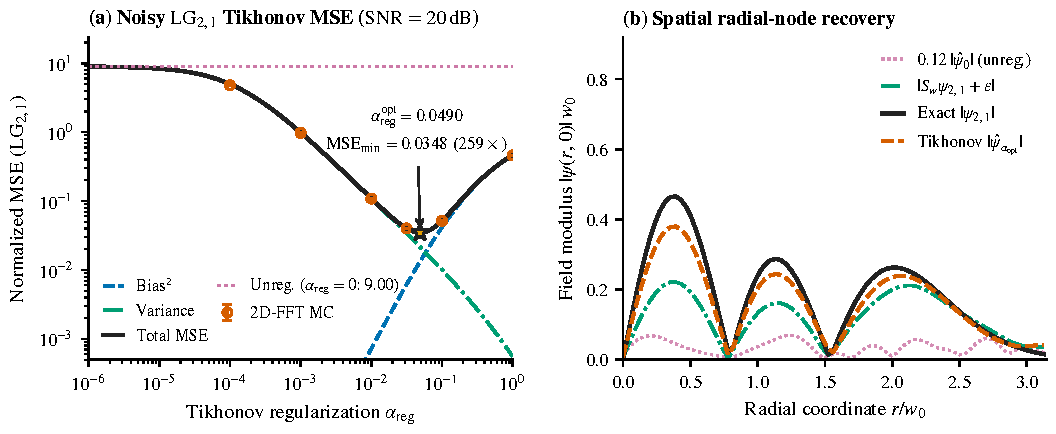
\includegraphics[width=0.94\textwidth]{figures/fig1_noisy_deconvolution.pdf}
\caption{Tikhonov-regularized PVB canonical dual reconstruction of noisy $\mathrm{LG}_{2,1}$ ($w/w_0 = 0.25$, $w k_{\max} = 3.0$, $P_\varepsilon = 0.01$, input $\mathrm{SNR} = 20\,\mathrm{dB}$). (a) Exact Parseval $\mathrm{Bias}^2$, variance, and total MSE [Eq.~\eqref{eq:tikhonov_mse_worked}] versus regularization weight $\alpha_{\mathrm{reg}}$ alongside $256\times 256$ 2D-FFT Monte Carlo trials (circles, $\pm 1\,\mathrm{SEM}$), reducing unregularized error $\mathrm{MSE}(0) = 9.002$ to $\mathrm{MSE}_{\min} = 0.03481$ at $\alpha_{\mathrm{reg}}^{\mathrm{opt}} = 0.04902$ [$258.6\times$ suppression, Eq.~\eqref{eq:mse_ratio_exact}]. (b) Single-realization radial field modulus $\abs{\psi(r,0)}\,w_0$ comparing exact $\mathrm{LG}_{2,1}$, frame-blurred noisy input $\abs{S_w\psi_{2,1}+\varepsilon}$, optimal Tikhonov recovery $\abs{\hat{\psi}_{\alpha_{\mathrm{opt}}}}$ restoring both radial nodes, and rescaled unregularized noise blow-up $0.12\,\abs{\hat{\psi}_0}$.}
\label{fig:noisy_deconv}
\end{figure*}

\subsection{Sturm--Liouville RCF Coupling and Multi-Ring SDM Equalization}
\label{subsec:rcf_sdm}

To model optical waveguide excitation from first principles, we solve the 1D scalar Helmholtz Sturm--Liouville radial eigenvalue problem (Appendix~\ref{app:methods}) for a step-index RCF with inner/outer core radii $r_1 = 6.0\,\mu\mathrm{m}$ and $r_2 = 9.0\,\mu\mathrm{m}$, silica cladding index $n_{\mathrm{clad}} = 1.444$, core-cladding contrast $\Delta n = 0.033$, and $\lambda = 1550\,\mathrm{nm}$—providing an exact boundary-value benchmark matched to the annular core dimensions of the graded-index (GRIN) RCF of Villalba \emph{et al.}~\cite{Villalba2023}. Launching unit-$L^2$-normalized physical PVBs ($\psi_{l,R}$ at $R = 7.5\,\mu\mathrm{m}$, $w = 1.72\,\mu\mathrm{m}$) yields modal power coupling $\eta_{\mathrm{PVB}}(l) = \abs{\braket{\psi_{\mathrm{RCF},l}}{\psi_{l,R}}}^2 \ge 95.87\%$ across all nine OAM orders $l = 0\text{--}8$, with mean efficiency $98.52\%$ and $\eta_{\mathrm{PVB}}(4) = 99.16\%$ (reaching mean $99.40\%$ at $w_{\mathrm{opt}} = 1.92\,\mu\mathrm{m}$) [Table~\ref{tab:rcf_coupling} and Fig.~\ref{fig:rcf_turbulence}(a)].

\begin{table}[t]
\caption{Exact Sturm--Liouville RCF power coupling efficiency $\eta_l$ ($r_1 = 6.0\,\mu\mathrm{m}$, $r_2 = 9.0\,\mu\mathrm{m}$, $n_{\mathrm{clad}} = 1.444$, $\Delta n = 0.033$, $\lambda = 1550\,\mathrm{nm}$) across OAM orders $l = 0\text{--}8$ for physical PVBs ($R = 7.5\,\mu\mathrm{m}$, $w = 1.72\,\mu\mathrm{m}$) versus $\mathrm{LG}_{0,l}$ at channel-matched ($w_0 = 4.50\,\mu\mathrm{m}$) and fixed-collimator ($w_0 = 3.22\,\mu\mathrm{m}$) waists, with last column $\Delta\eta_{\mathrm{fix}} = 10\log_{10}(\eta_{\mathrm{PVB}}/\eta_{\mathrm{LG},3.22})$.}
\label{tab:rcf_coupling}
\begin{ruledtabular}
\setlength{\tabcolsep}{3.2pt}
\begin{tabular}{ccccc}
$l$ & $\eta_{\mathrm{PVB}}$ & $\eta_{\mathrm{LG}}$ ($4.50\,\mu\mathrm{m}$) & $\eta_{\mathrm{LG}}$ ($3.22\,\mu\mathrm{m}$) & $\Delta\eta_{\mathrm{fix}}$ (dB) \\
\hline
0 & 0.9931 & 0.0528 & 0.0041 & $+23.87$ \\
1 & 0.9932 & 0.1999 & 0.0193 & $+17.12$ \\
2 & 0.9934 & 0.4204 & 0.0539 & $+12.66$ \\
3 & 0.9931 & 0.6464 & 0.1145 & $+9.38$ \\
4 & 0.9916 & 0.8115 & 0.2026 & $+6.90$ \\
5 & 0.9883 & 0.8842 & 0.3134 & $+4.99$ \\
6 & 0.9825 & 0.8707 & 0.4371 & $+3.52$ \\
7 & 0.9733 & 0.7996 & 0.5617 & $+2.39$ \\
8 & 0.9587 & 0.7054 & 0.6758 & $+1.52$ \\
\end{tabular}
\end{ruledtabular}
\end{table}

Table~\ref{tab:rcf_coupling} contrasts $\eta_{\mathrm{PVB}}$ against two physically distinct $\mathrm{LG}_{0,l}$ launch conventions: (i) a fixed-collimator multi-channel setup ($w_0 = 3.22\,\mu\mathrm{m}$, calibrated to a single-mode-fed SLM launch), where $l$-dependent expansion places the $\mathrm{LG}_{0,4}$ ring peak at $r_{\mathrm{peak}} = w_0\sqrt{2} = 4.55\,\mu\mathrm{m}$ inside the inner core boundary ($\eta_{\mathrm{LG}} = 0.2026$), yielding an analytical $+6.90\,\mathrm{dB}$ PVB coupling gain at $l = 4$ that closely parallels the experimental $+6.83\,\mathrm{dB}$ GRIN-RCF gain measured in Ref.~\cite{Villalba2023}; and (ii) an $l = 4$ channel-matched waist ($w_0 = 4.50\,\mu\mathrm{m}$, $r_{\mathrm{peak}} = 6.36\,\mu\mathrm{m}$), which lifts $\eta_{\mathrm{LG}}(4)$ to $0.8115$ ($+0.87\,\mathrm{dB}$ PVB gain) but severely mismatches low OAM channels ($\eta_{\mathrm{LG}}(1) = 0.1999$) and higher orders ($\eta_{\mathrm{LG}}(9) = 0.589$, dropping to $0.355$ by $l = 11$).

In free-space or large-core multi-ring SDM links, $N$ concentric radial PVB channels at fixed $l$ spaced by $\Delta R \ge 2.0\,w$ can be passively demultiplexed using unitary MPLC phase cascades~\cite{Fontaine2019} or log-polar coordinate transformers paired with refractive radial mode sorters~\cite{Berkhout2010,Bouchard2018}, followed by $N \times N$ linear zero-forcing (ZF) equalization~\cite{Willner2015,Wang2019,Proakis2008} with $(\gamma^{-1})_{nm}$. Under frame-correlated optical-amplifier noise ($\mathbb{E}[\boldsymbol{\varepsilon}\boldsymbol{\varepsilon}^\dagger] = \sigma^2\gamma$) and post-detection receiver AWGN ($\mathbb{E}[\boldsymbol{\varepsilon}\boldsymbol{\varepsilon}^\dagger] = \sigma^2 I_N$), the per-channel SNR noise-enhancement penalties are
\begin{equation}
\mathcal{P}_{\mathrm{corr}} = \frac{1}{N}\operatorname{Tr}(\gamma^{-1}), \qquad \mathcal{P}_{\mathrm{AWGN}} = \frac{1}{N}\operatorname{Tr}(\gamma^{-2}).
\label{eq:zf_penalties}
\end{equation}
For $N = 6$ concentric rings at $\Delta R = 2.0\,w$ ($\kappa(\gamma) = 1.645$, $17.36\,\mathrm{dB}$ adjacent power isolation~\cite{AyalaPaperI}), Eq.~\eqref{eq:zf_penalties} gives $\mathcal{P}_{\mathrm{corr}} = 1.032$ ($0.14\,\mathrm{dB}$) and $\mathcal{P}_{\mathrm{AWGN}} = 1.099$ ($0.41\,\mathrm{dB} \le 0.42\,\mathrm{dB}$), falling to $0.01\,\mathrm{dB}$ and $0.04\,\mathrm{dB}$ at $\Delta R = 2.5\,w$. Figure~\ref{fig:rcf_turbulence}(a, inset) plots the resulting dispersion-free $l = 4$ on-off keying (OOK) bit-error rate $\mathrm{BER} = \frac{1}{2}\operatorname{erfc}(\sqrt{\eta_l (E_b/N_0)/(2\mathcal{P})})$ versus pre-coupling $E_b/N_0$, confirming negligible multi-ring equalization penalty.

\begin{figure*}[t]
\centering
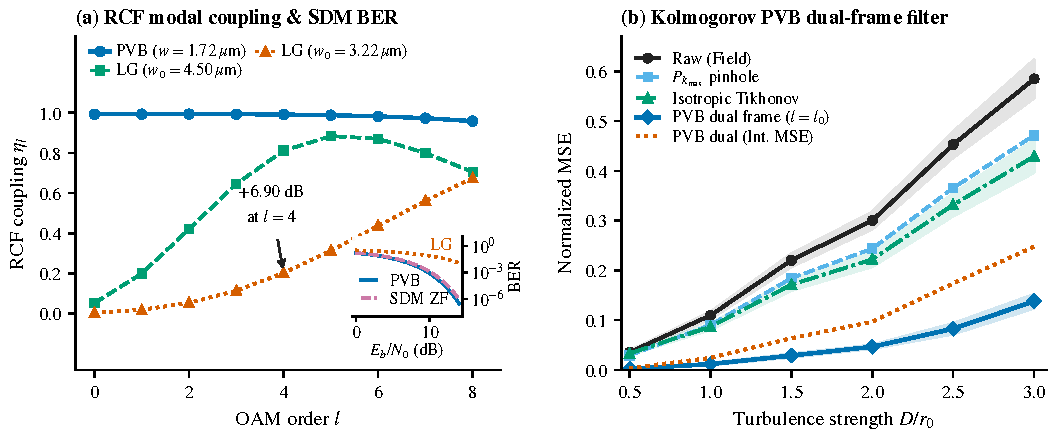
\includegraphics[width=0.94\textwidth]{figures/fig2_rcf_turbulence.pdf}
\caption{Classical waveguide coupling and turbulent free-space spatial filtering. (a) Step-index Sturm--Liouville RCF coupling $\eta_l$ (Table~\ref{tab:rcf_coupling}) for physical PVBs ($w = 1.72\,\mu\mathrm{m}$, mean $0.9852$) versus $\mathrm{LG}_{0,l}$ at $w_0 = 4.50\,\mu\mathrm{m}$ and $w_0 = 3.22\,\mu\mathrm{m}$ ($+6.90\,\mathrm{dB}$ gain at $l = 4$); inset shows dispersion-free $l = 4$ OOK BER versus pre-coupling $E_b/N_0$ (dB) including the $0.41\,\mathrm{dB}$ ($N = 6$) AWGN ZF penalty at $\Delta R = 2.0\,w$. (b) Normalized field MSE ($\pm 1\,\mathrm{SEM}$) across $40$ subharmonic Kolmogorov phase screens ($D_{\mathrm{ap}} = 3.0\,\mathrm{mm}$, $z = 0.5\,\mathrm{m}$, Table~\ref{tab:kolmogorov}) comparing raw distortion, circular pinhole $P_{k_{\max}}$, isotropic Tikhonov ($\alpha_{\mathrm{reg}} = 0.0183$), and the single-OAM discrete radial PVB dual-frame projector ($l_0 = 1, N = 5$), alongside PVB dual-frame intensity MSE (dotted).}
\label{fig:rcf_turbulence}
\end{figure*}

\section{Classical Photonics II: Single-OAM Discrete PVB Dual-Frame Filtering in Kolmogorov Turbulence}
\label{sec:turbulence}

Atmospheric refractive-index turbulence scatters structured OAM beams simultaneously into high-$k_\perp$ radial speckles and neighboring azimuthal OAM sectors $l \neq l_0$~\cite{Paterson2005,TylerBoyd2009,AndrewsPhillips2005}. Crucially, rotationally symmetric Fourier filters—such as the circular Paley--Wiener low-pass pinhole $P_{k_{\max}}$ or the isotropic Tikhonov filter $S_{w,\alpha_{\mathrm{reg}}}^{-1}S_w$ ($\alpha_{\mathrm{reg}} = e^{-(w k_{\max})^2} = 0.0183$)—attenuate only $k_\perp > k_{\max}$ speckles while leaving low-order non-axisymmetric aberrations (tilt, astigmatism, coma) and all $l \neq l_0$ OAM crosstalk untouched.

To exploit the azimuthal--radial structure of PVB frames directly, we project the received turbulent field $\psi_{\mathrm{turb}}$ onto the propagated single-OAM discrete radial PVB subspace $\operatorname{span}\{\psi_{l_0,R_n}^{(\mathrm{prop})}\}_{n=1}^N$ ($l_0 = 1$, $N = 5$ concentric rings $R_n \in \{0.25, 0.625, 1.00, 1.375, 1.75\}\,\mathrm{mm}$ with $\Delta R = 1.5\,w$, unit-normalized Gram condition number $\kappa(\gamma) = 10.12$, realizable optically via an $l_0$ spiral phase fork and radial MPLC sorter) using the exact biorthogonal dual-frame inverse $(\gamma^{-1})_{nm}$:
\begin{equation}
P_{\mathrm{PVB},l_0}\psi_{\mathrm{turb}} = \sum_{n,m=1}^N (\gamma^{-1})_{nm}\braket{\psi_{l_0,R_m}^{(\mathrm{prop})}}{\psi_{\mathrm{turb}}}\psi_{l_0,R_n}^{(\mathrm{prop})}.
\label{eq:discrete_pvb_turb_filter}
\end{equation}
We simulate $40$ independent $256\times 256$ subharmonic-corrected Kolmogorov phase screens~\cite{Lane1992} ($D_{\mathrm{ap}} = 3.0\,\mathrm{mm}$, propagation distance $z = 0.5\,\mathrm{m}$, signal PVB $R_0 = 1.0\,\mathrm{mm}$, $w = 0.25\,\mathrm{mm}$, $k_{\max} = 8.0\,\mathrm{rad/mm}$) across Fried turbulence strengths $D/r_0 \in [0.5, 3.0]$. Table~\ref{tab:kolmogorov} and Fig.~\ref{fig:rcf_turbulence}(b) demonstrate that at $D/r_0 = 3.0$, where $44.8\%$ of total beam power scatters outside the $l_0 = 1$ radial-PVB subspace, isotropic $P_{k_{\max}}$ and Tikhonov filters reduce normalized field MSE modestly from $0.585$ to $0.471$ and $0.429$, whereas the single-OAM PVB dual-frame projector~\eqref{eq:discrete_pvb_turb_filter} suppresses field MSE by $4.24\times$ to $0.138$ (and intensity MSE from $0.553$ to $0.248$).

\begin{table}[t]
\caption{Normalized field MSE (mean $\pm 1\,\mathrm{SEM}$ over $40$ subharmonic Kolmogorov screens) across turbulence strength $D/r_0$, comparing raw turbulent distortion, circular pinhole $P_{k_{\max}}$, isotropic Tikhonov, and single-OAM discrete PVB dual-frame projection $P_{\mathrm{PVB},l_0}$ [Eq.~\eqref{eq:discrete_pvb_turb_filter}], alongside scattered out-of-subspace power fraction $f_{\mathrm{out}}$.}
\label{tab:kolmogorov}
\begin{ruledtabular}
\footnotesize
\setlength{\tabcolsep}{1.8pt}
\begin{tabular}{cccccc}
$D/r_0$ & $f_{\mathrm{out}}$ & Raw & $P_{k_{\max}}$ & Tikhonov & PVB Dual \\
\hline
0.5 & $3.1\%$ & $0.036\pm 0.003$ & $0.029$ & $0.033$ & $0.0022\pm 0.0003$ \\
1.0 & $9.7\%$ & $0.110\pm 0.007$ & $0.090$ & $0.087$ & $0.0117\pm 0.0019$ \\
1.5 & $19.4\%$ & $0.220\pm 0.013$ & $0.184$ & $0.171$ & $0.0288\pm 0.0035$ \\
2.0 & $27.0\%$ & $0.300\pm 0.017$ & $0.244$ & $0.222$ & $0.0465\pm 0.0037$ \\
2.5 & $36.2\%$ & $0.453\pm 0.026$ & $0.365$ & $0.332$ & $0.0827\pm 0.0106$ \\
3.0 & $44.8\%$ & $0.585\pm 0.039$ & $0.471$ & $0.429$ & $0.1379\pm 0.0139$ \\
\end{tabular}
\end{ruledtabular}
\end{table}

\section{Quantum Photonics: Multi-Plane Gouy IC-POVM Tomography and Iris Invariance}
\label{sec:quantum}

\subsection{Passive Multi-Plane Gouy-Diverse Radial-Qudit IC-POVM}
\label{subsec:povm}

Consider quantum state tomography on a $d$-dimensional fixed-$l$ radial photonic qudit space $\mathcal{H}_d^{(l)} = \operatorname{span}\{\ket{\psi_{p,l}}\}_{p=0}^{d-1}$. Single-plane ($z = 0$) PVB ring-intensity projections are \emph{not} informationally complete (IC): because $c_{l,p}(R) \in \mathbb{R}$ in Eq.~\eqref{eq:c_lp_recap}, single-plane projectors $\ket{\Phi_{l,R}}\bra{\Phi_{l,R}}$ have real matrix elements in the $\mathrm{LG}_{p,l}$ basis and vanish on all $d(d-1)/2$ imaginary antisymmetric coherences, spanning at most $2d - 1 < d^2$ real Hermitian parameters (certified rank $7/16$ at $d = 4$, $l = 1$).

We lift this real-polynomial degeneracy passively by splitting the input beam across $M \ge d+1$ propagation planes $z_m$ (realizable without active SLM switching via a passive beam-splitter tree or multi-plane light converter~\cite{Fontaine2019,Bouchard2018}) sampling distinct Gouy phases $\vartheta_m = \arctan(z_m/z_R)$, where $z_R = k_0 w_0^2/2$. Because at plane $z_m \neq 0$ each $\mathrm{LG}_{p,l}$ basis mode expands radially by $\sigma_m = \sqrt{1 + (z_m/z_R)^2}$ and acquires spherical wavefront curvature radius $R_c(z_m) = z_m[1 + (z_R/z_m)^2]$, each plane-$z_m$ PVB analyzer is radially rescaled as $(R_{m,k}, w_m) = \sigma_m(R_k, w)$ and wavefront-compensated by a thin lens of focal length $f_m = R_c(z_m)$, defining $\phi_{m,k}(r,\phi) = \sigma_m^{-1} e^{ik_0 r^2/[2R_c(z_m)]}\,\Phi_{l,\sigma_m R_k}(r,\phi;\,\sigma_m w)$. Changing radial variables $r' = r/\sigma_m$ yields the exact POVM elements~\cite{Renes2004}
\begin{align}
\Pi_{m,k} &= \frac{R_k \Delta R}{M}\ket{\phi_{m,k}}\bra{\phi_{m,k}}, \nonumber \\
\braket{\psi_{p,l}(z_m)}{\phi_{m,k}} &= e^{-i(2p+\abs{l}+1)\vartheta_m} c_{l,p}(R_k),
\label{eq:ic_povm_elements}
\end{align}
completed on $\mathcal{H}_d^{(l)}$ by the positive semidefinite residual element $\Pi_{\mathrm{res}} = I_d - \sum_{m,k}\Pi_{m,k}$ ($\lambda_{\max}(\sum \Pi_{m,k}) = 0.9050 < 1$, enabled directly by the Bessel bound $B = 1$ of Paper~I~\cite{AyalaPaperI}).

For $d = 4$ ($d^2 = 16$), $l = 1$, $w/w_0 = 0.25$, $M = 5$ planes ($\vartheta_m$ uniformly spaced on $[0, 0.45\pi]$), and $40$ midpoint radial bins $R_k \in (0, 3.5\,w_0]$, Eq.~\eqref{eq:ic_povm_elements} achieves full IC rank $16/16$, operator-frame condition numbers $\kappa(\mathcal{S}_{\mathrm{POVM}}) = 442.5$ on $\mathrm{Herm}(\mathcal{H}_4)$ and $\kappa_{\mathrm{Bloch}}(\mathcal{S}_{\mathrm{POVM}}) = 88.3$ on the $15$-dimensional traceless Bloch subspace (Appendix~\ref{app:methods}), classical Fisher condition number $\kappa(\mathbf{F}) = 14.86$ ($\lambda_{\min}(\mathbf{F}) = 0.1261$), and single-photon Cram\'er--Rao bound (CRB) at $\rho_0 = I_4/4$:
\begin{equation}
\operatorname{Tr}\!\left(\mathbf{F}^{-1}\right) = 41.80 \quad (\text{with }\Pi_{\mathrm{res}};\; 42.96\text{ without}),
\label{eq:fisher_crb}
\end{equation}
compared against $18.75$ for $5$ sequential mutually unbiased bases (MUBs)—trading a $2.23\times$ photon-budget factor for completely passive, reconfiguration-free single-shot acquisition. Iterative $R\hat{\rho}R$ maximum-likelihood estimation (MLE)~\cite{Lvovsky2004} over $30$ Poisson/multinomial trials per photon budget converges cleanly to the asymptotic CRB $41.80/N_{\mathrm{phot}}$ [Table~\ref{tab:povm_mle} and Fig.~\ref{fig:quantum_utility}(a)].

\begin{table}[t]
\caption{Frobenius reconstruction error $\norm{\hat{\rho} - \rho_0}_F^2$ (mean $\pm 1\,\mathrm{SEM}$ across $30$ trials) for passive single-shot $M = 5$ Gouy-diverse PVB IC-POVM $R\hat{\rho}R$ MLE versus sequential $5$-MUB MLE at $\rho_0 = I_4/4$ ($d = 4, l = 1, w/w_0 = 0.25$), compared against the asymptotic CRB $41.80/N_{\mathrm{phot}}$.}
\label{tab:povm_mle}
\begin{ruledtabular}
\setlength{\tabcolsep}{4pt}
\begin{tabular}{cccc}
$N_{\mathrm{phot}}$ & PVB CRB & PVB $R\hat{\rho}R$ MLE & $5$-MUB MLE \\
\hline
$300$ & $0.1393$ & $0.1294\pm 0.0068$ & $0.0571\pm 0.0032$ \\
$1{,}000$ & $0.0418$ & $0.0350\pm 0.0027$ & $0.0173\pm 0.0011$ \\
$3{,}000$ & $0.0139$ & $0.0146\pm 0.0012$ & $0.0062\pm 0.0005$ \\
$10{,}000$ & $0.0042$ & $0.0035\pm 0.0002$ & $0.0019\pm 0.0001$ \\
$30{,}000$ & $0.0014$ & $0.0013\pm 0.0001$ & $0.00061\pm 0.00004$ \\
\end{tabular}
\end{ruledtabular}
\end{table}

\begin{figure*}[t]
\centering
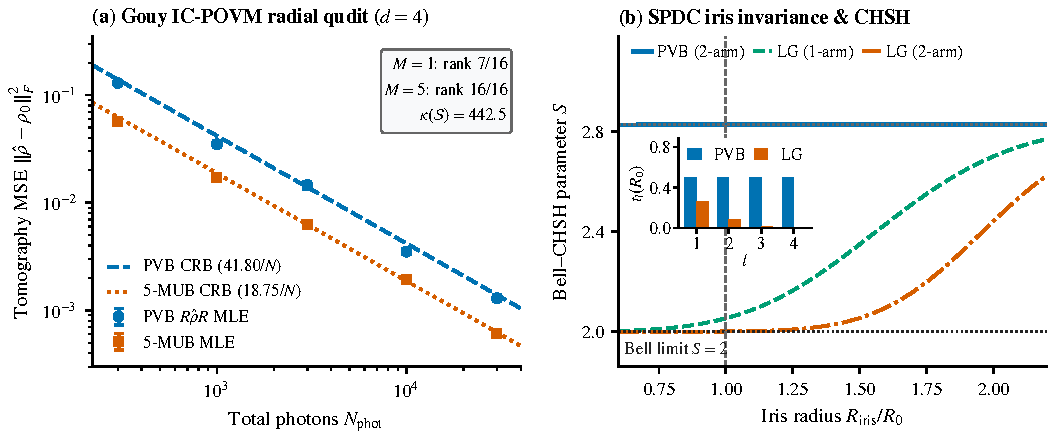
\includegraphics[width=0.94\textwidth]{figures/fig3_quantum_tomography_chsh.pdf}
\caption{Quantum state tomography and circular-iris entanglement preservation. (a) Passive $M = 5$ Gouy-diverse IC-POVM radial-qudit tomography ($d = 4, l = 1, w/w_0 = 0.25$, full rank $16/16$ versus $7/16$ at $M = 1$, $\kappa(\mathcal{S}_{\mathrm{POVM}}) = 442.5$): $30$-trial $R\hat{\rho}R$ MLE MSE (Table~\ref{tab:povm_mle}) tracks the single-photon CRB $41.80/N_{\mathrm{phot}}$ alongside sequential $5$-MUB tomography ($18.75/N_{\mathrm{phot}}$). (b) Post-selected SPDC Bell--CHSH parameter $S(R_{\mathrm{iris}}/R_0)$ [Eq.~\eqref{eq:iris_chsh}] for $\ket{\Psi} = (\ket{1,-1}+\ket{4,-4})/\sqrt{2}$ ($w = 0.1\,R_0$, LG $w_0 = \sqrt{2}\,R_0$); inset compares single-mode transmissions $t_{1..4}(R_0)$.}
\label{fig:quantum_utility}
\end{figure*}

\subsection{\texorpdfstring{$l$}{l}-Invariant QKD Footprint and Leading-Order Circular-Iris Bell--CHSH Protection}
\label{subsec:spdc_chsh}

In high-dimensional OAM QKD and spontaneous parametric down-conversion (SPDC) links~\cite{Cerf2002,Mirhosseini2015,LawEberly2004,Walborn2010}, a finite circular pupil $\hat{T}_{\mathrm{iris}} = \Theta(R_{\mathrm{iris}} - r)$ attenuates single-mode $\mathrm{LG}_{0,l}$ detection probabilities according to the regularized lower incomplete gamma function $t_l^{\mathrm{LG}}(R_{\mathrm{iris}}) = \braket{\psi_{0,l}}{\hat{T}_{\mathrm{iris}}\psi_{0,l}} = P(\abs{l}+1, 2R_{\mathrm{iris}}^2/w_0^2)$, opening severe $l$-dependent detection-efficiency side-channels and Procrustean entanglement degradation.

By contrast, unit-normalized physical PVBs preserve pupil transmission $t_l^{\mathrm{PVB}}(R_{\mathrm{iris}}) = \braket{\psi_{l,R_0}}{\hat{T}_{\mathrm{iris}}\psi_{l,R_0}}$ to leading order in $w/R_{\mathrm{iris}}$. At $R_{\mathrm{iris}} = R_0$ with $w = 0.1\,R_0$ (versus $l=1$ peak-matched $\mathrm{LG}_{0,l}$ with $w_0 = \sqrt{2}\,R_0$), exact quadrature gives $t_{1..4}^{\mathrm{PVB}}(R_0) = [0.49992, 0.49962, 0.49912, 0.49841]$ versus $t_{1..4}^{\mathrm{LG}}(R_0) = [0.26424, 0.08030, 0.01899, 0.00366]$ [Fig.~\ref{fig:quantum_utility}(b) inset]. For the two-photon OAM Bell state $\ket{\Psi} = (\ket{1,-1} + \ket{4,-4})/\sqrt{2}$, post-selected single-mode projection behind circular irises yields the Bell--CHSH parameter~\cite{Clauser1969}
\begin{equation}
S(R_{\mathrm{iris}}) = 2\sqrt{1 + \mathcal{V}^2(R_{\mathrm{iris}})}, \qquad \mathcal{V} = \frac{2\sqrt{t_1 t_4}}{t_1 + t_4},
\label{eq:iris_chsh}
\end{equation}
for one-arm truncation (with $t_l \mapsto t_l^2$ for symmetric two-arm irises). As shown asymptotically in Appendix~\ref{app:methods}, the relative transmission imbalance at $R_{\mathrm{iris}} = R_0$ scales as $\abs{t_{l_1}^{\mathrm{PVB}} - t_{l_2}^{\mathrm{PVB}}}/(t_{l_1}^{\mathrm{PVB}} + t_{l_2}^{\mathrm{PVB}}) = \mathcal{O}(\abs{l_1^2 - l_2^2}(w/R_0)^3)$, bounding the CHSH deviation from Tsirelson's bound $2\sqrt{2} \approx 2.8284271$ at sixth order in $w/R_0$:
\begin{equation}
0 < 2\sqrt{2} - S_{\mathrm{PVB}}(R_0) = \mathcal{O}\!\left((l_1^2 - l_2^2)^2 \left(\frac{w}{R_0}\right)^6\right).
\label{eq:chsh_error_bound}
\end{equation}
At $w = 0.1\,R_0$ and $R_{\mathrm{iris}} = R_0$, exact quadrature yields $S_{\mathrm{PVB}}^{(1)}(R_0) = 2.8284255$ ($2\sqrt{2} - S_{\mathrm{PVB}}^{(1)} = 1.62\times 10^{-6}$) for one-arm truncation and $S_{\mathrm{PVB}}^{(2)}(R_0) = 2.8284206$ ($2\sqrt{2} - S_{\mathrm{PVB}}^{(2)} = 6.48\times 10^{-6}$) for two-arm truncation, alongside a $24.92\%$ two-photon coincidence survival probability—whereas $\mathrm{LG}$ modes collapse to $S_{\mathrm{LG}}^{(1)}(R_0) = 2.0532$ and $S_{\mathrm{LG}}^{(2)}(R_0) = 2.0008$ ($3.49\%$ coincidence survival, with $\ket{4,-4}$ attenuated to $t_4^2 = 1.3\times 10^{-5}$) [Fig.~\ref{fig:quantum_utility}(b)].

\section{Conclusions}
\label{sec:conclusions}

Applying the continuous Hilbert-frame operator theory of Paper~I~\cite{AyalaPaperI}, we have demonstrated five quantitative classical and quantum photonic protocols enabled by finite-width physical PVBs: (i) $258.6\times$ ($24.1\,\mathrm{dB}$) MSE suppression in noisy $\mathrm{LG}_{2,1}$ reconstruction via the Tikhonov-regularized canonical dual frame; (ii) $98.52\%$ mean Sturm--Liouville RCF coupling across $l = 0\text{--}8$ ($+6.90\,\mathrm{dB}$ gain over fixed-collimator $\mathrm{LG}_{0,4}$) paired with $\le 0.42\,\mathrm{dB}$ zero-forcing equalization penalty for $N = 6$ concentric radial SDM channels at $\Delta R = 2.0\,w$; (iii) $4.24\times$ field-MSE reduction in Kolmogorov atmospheric turbulence via single-OAM discrete PVB dual-frame projection; (iv) passive single-shot $M = 5$ Gouy-diverse IC-POVM tomography of $d = 4$ radial qudits achieving full rank $16/16$ and $\operatorname{Tr}(\mathbf{F}^{-1}) = 41.80$; and (v) leading-order circular-iris Bell--CHSH entanglement protection with sixth-order $(w/R_0)^6$ Tsirelson-bound deviation. Together with Paper~I, these results establish physical PVB frames as a rigorous, experimentally accessible architecture for high-dimensional spatial-mode photonics.

\begin{acknowledgments}
AI disclosure: Portions of this work were developed with the assistance of Gemini~4~Carbon (Google DeepMind) operating within the Antigravity IDE (accessed November 2026). The AI was used for symbolic calculus, asymptotic expansions, numerical simulation scripting, and \LaTeX{} typesetting. All hypotheses, boundary-value models, proofs, and physical interpretations were conceived and audited by the human author, Sebasti\'an Ayala, who takes full responsibility for the integrity and accuracy of the manuscript in accordance with American Physical Society editorial policies.
\end{acknowledgments}

\section*{Data Availability}
All optical simulation scripts (\texttt{pvb\_\allowbreak physics.py}, \texttt{verify\_\allowbreak analytical\_\allowbreak tables.py}, and \texttt{generate\_\allowbreak figures.py}) and numerical benchmark datasets (\texttt{verified\_\allowbreak metrics.json}) supporting the findings of this study are self-contained and openly available from the author upon reasonable request and in the accompanying open-source code distribution.

\appendix

\section{Sturm--Liouville RCF Solver, IC-POVM Superoperator, and Circular-Iris Asymptotics}
\label{app:methods}

\paragraph*{Step-index RCF Sturm--Liouville eigenmodes.}
Under the weakly guiding scalar Helmholtz approximation ($\Delta n / n_{\mathrm{clad}} = 0.0229 \ll 1$), guided RCF eigenmodes $\psi_{\mathrm{RCF},l}(r,\phi) = (2\pi)^{-1/2} u_l(r) e^{il\phi}$ satisfy
\begin{equation}
-\frac{1}{r}\frac{d}{dr}\!\left(r\frac{du_l}{dr}\right) + \left[\frac{l^2}{r^2} - k_0^2 n^2(r)\right] u_l(r) = -\beta_l^2 u_l(r),
\label{eq:app_sl_ode}
\end{equation}
with $n(r) = n_{\mathrm{clad}} + \Delta n$ for $r \in [r_1, r_2]$ and $n_{\mathrm{clad}}$ elsewhere, subject to regularity $u_l(r) \propto I_{\abs{l}}(\kappa_l r)$ on $[0,r_1]$ and evanescent decay $u_l(r) \propto K_{\abs{l}}(\kappa_l r)$ on $[r_2,\infty)$ ($\kappa_l = \sqrt{\beta_l^2 - k_0^2 n_{\mathrm{clad}}^2}$). Matching $u_l$ and $du_l/dr$ across $r_1$ and $r_2$ yields a $4\times 4$ Bessel determinant whose fundamental radial root $\beta_l$ gives the unit-norm guided mode ($\int_0^\infty \abs{u_l(r)}^2 r\,dr = 1$) used in Table~\ref{tab:rcf_coupling}.

\paragraph*{IC-POVM operator frame and Fisher matrix.}
Let $\{B_\mu\}_{\mu=0}^{d^2-1}$ be an orthonormal Hermitian operator basis on $\mathcal{H}_d^{(l)}$ with $B_0 = I_d/\sqrt{d}$ and traceless generalized Gell-Mann generators $\{B_j\}_{j=1}^{d^2-1}$ ($\operatorname{Tr}(B_\mu B_\nu) = \delta_{\mu\nu}$). For POVM outcomes $\{\Pi_\alpha\} = \{\Pi_{m,k}\} \cup \{\Pi_{\mathrm{res}}\}$, the POVM frame superoperator on $\mathrm{Herm}(\mathcal{H}_d^{(l)})$ has matrix $[\mathcal{S}_{\mathrm{POVM}}]_{\mu\nu} = \sum_\alpha \operatorname{Tr}(\Pi_\alpha B_\mu)\operatorname{Tr}(\Pi_\alpha B_\nu)$, with condition number $\kappa(\mathcal{S}_{\mathrm{POVM}}) = \lambda_{\max}(\mathcal{S}_{\mathrm{POVM}})/\lambda_{\min}(\mathcal{S}_{\mathrm{POVM}}) = 442.5$ (and $\kappa_{\mathrm{Bloch}} = 88.3$ on the $15\times 15$ traceless block $1 \le j,k \le 15$). Parameterizing $\rho(\boldsymbol{\theta}) = I_d/d + \sum_{j=1}^{d^2-1}\theta_j B_j$, single-photon outcome probabilities $p_\alpha(\boldsymbol{\theta}) = \operatorname{Tr}[\rho(\boldsymbol{\theta})\Pi_\alpha]$ yield the $(d^2-1)\times(d^2-1)$ classical Fisher information matrix at $\boldsymbol{\theta} = \mathbf{0}$ ($\rho_0 = I_d/d$):
\begin{equation}
F_{jk} = \sum_\alpha \frac{\operatorname{Tr}(\Pi_\alpha B_j)\operatorname{Tr}(\Pi_\alpha B_k)}{\operatorname{Tr}(\Pi_\alpha)/d},
\label{eq:app_fisher}
\end{equation}
giving $\operatorname{Tr}(\mathbf{F}^{-1}) = 41.80$ in Eq.~\eqref{eq:fisher_crb}.

\paragraph*{Leading-order circular-iris CHSH asymptotics.}
Expanding $\abs{\psi_{l,R_0}(r)}^2$ around $r = R_0$ via Hankel's series for $I_{\abs{l}}(2R_0 r/w^2)$ and $I_{\abs{l}}(R_0^2/w^2)$ for $w \ll R_0$ gives $t_l^{\mathrm{PVB}}(R_0) = \int_0^{R_0}\abs{\psi_{l,R_0}(r)}^2 2\pi r\,dr = \frac{1}{2} + c_0(w/R_0) - [(4l^2 - 1)/(16\sqrt{2\pi})](w/R_0)^3 + \mathcal{O}((w/R_0)^5)$, where $c_0$ is independent of $l$. Hence $\delta_{14} \equiv (t_1^{\mathrm{PVB}} - t_4^{\mathrm{PVB}})/(t_1^{\mathrm{PVB}} + t_4^{\mathrm{PVB}}) \approx [15/(4\sqrt{2\pi})](w/R_0)^3 = 1.496\times 10^{-3}$ at $w/R_0 = 0.1$ (matching the exact quadrature value $1.510\times 10^{-3}$ to $<1\%$). Since $\mathcal{V} = \sqrt{1 - \delta_{14}^2} \approx 1 - \frac{1}{2}\delta_{14}^2$ for one-arm truncation (and $\sqrt{1 - [2\delta_{14}/(1+\delta_{14}^2)]^2} \approx 1 - 2\delta_{14}^2$ for two-arm truncation), Eq.~\eqref{eq:iris_chsh} gives $2\sqrt{2} - S_{\mathrm{PVB}}^{(1)}(R_0) \approx (\delta_{14}^2/\sqrt{2}) = 1.58\times 10^{-6}$ and $2\sqrt{2} - S_{\mathrm{PVB}}^{(2)}(R_0) \approx 2\sqrt{2}\,\delta_{14}^2 = 6.33\times 10^{-6}$, in quantitative agreement with the exact quadrature values $1.62\times 10^{-6}$ and $6.48\times 10^{-6}$ in Eq.~\eqref{eq:chsh_error_bound}.

\bibliography{references}

\end{document}
